\documentclass{mcmthesis}
\mcmsetup{CTeX = false,   % 使用 CTeX 套装时,设置为 true
	tcn = 78435, problem = E,
	sheet = true, titleinsheet = true, keywordsinsheet = true,
	titlepage = false, abstract = true}
\usepackage{palatino}
\usepackage{float}
\usepackage{etoc}
\usepackage{array}
\usepackage{setspace}
\usepackage{titletoc}
\newcolumntype{I}{!{\vrule width 3pt}}
\newlength\savedwidth
\newcommand\whline{\noalign{\global\savedwidth\arrayrulewidth
		\global\arrayrulewidth 1.2pt}%
	\hline
	\noalign{\global\arrayrulewidth\savedwidth}}
\newlength\savewidth
\newcommand\shline{\noalign{\global\savewidth\arrayrulewidth
		\global\arrayrulewidth 1.2pt}%
	\hline
	\noalign{\global\arrayrulewidth\savewidth}}
\title{Climate Change, Regional Fragility Variation and Human Intervention}
\author{}
\date{}
\begin{document}
	\begin{abstract}
		To define a country's \textbf{fragility}, we can focus on several specific issues. In this paper, we are going to analyze the relationship between climate change and regional fragility.
		
		First, we establish a model without climate change to see the trend of a country’s fragility in a few years. Using the logic of \textbf{Principal Component Analysis}, we come up with some influence factors that occur in most countries. We assume the fragility to obey \textbf{Markov Chain} if there are no climate influences and external interventions. Then we modify the model with climate change and other detailed factors. After that, we run our model on three countries which are respectively accepted as stable, vulnerable and fragile to set the evaluation standard.
		
		Second, we plan to run the model on a country at the edge of breakdown. Central African Republic ranks third on Fragile States Index database and is currently affected by climate change. We iterate our model to predict the fragility of Central African Republic in several years, and separately give random climate change and harmful climate change to see the trends.
		
		Third, our attention is focused on a country which is rather stable: the Netherlands. We refine our model with more specific climate change in this country, use \textbf{Fixed Point Iteration} to find the tipping point, and obtain the climate change types that influence the Netherlands most from the calculation. After this, we specify the policies their government can implement, and make more detailed modifications on our prediction model to calculate the efficiency of these policies. The government should make special efforts on the most effective policy.
		
		Finally, we do the universality analysis of our model, finding that for smaller “states” and larger “states”, there should be some small modification as well. The core of this model remains the same, so if we want to run this model on other situations, there should be some background study initially.		
		
		\begin{keywords}
			Climate change; Fragility analysis; Principal Component Analysis; Markov Chain; Fixed Point Iteration
		\end{keywords}
	\end{abstract}
	\maketitle
	

	
	\newpage
	\begin{center}
		\tableofcontents
		%\setcounter{page}{0}
		%\thispagestyle{empty}
	\end{center}
	\newpage
	
	\section{Introduction}
	
	A \textbf{fragile state} is a low-income country or a sovereign state that is characterized by weak state capacity and/or weak state legitimacy[1]. It increases the vulnerability of citizens towards a range of shocks, including economic fluctuation, political upheaval, and so forth. 
	
	Particularly, \textbf{climate shock} such as unpredictable natural disasters, extreme weather, decreasing cultivated land and changing ranges of plants and animals may dramatically aggravate fragile states and may further leads to regional violent conflicts when social fragmentation and weak governance exist as well. Therefore, it is of vital significance to research on how climate change will affect the instability or fragility of a state and how human intervention can mitigate such negative impact.
	
	In this paper, we mainly focus on analyzing the influence of climate change on regional instability and fragility. More specifically, we pay attention to the following issues:
	\begin{itemize}
		\item Develop a model that determines the fragility of a country and identify when a state is fragile, vulnerable, or stable. Simultaneously, the model will measure the impact of climate change and analyze direct and indirect means by which climate change increases the fragility.
		\item Select Central African Republic, one of the top 10 most fragile states as determined by the Fragile State Index (http://fundforpeace.org/fsi/data/) and use the model to analyze how climate change has increased the fragility of it and show in what way(s) Central African Republic may be less fragile without these effects.
		\item Apply the model on the Netherlands to measure its fragility, and determine in what way and when climate change may increase the fragility of the state. Identify any definitive indicators. Define a tipping point and predict when the Netherlands may reach it.
		\item Use the model to show which state driven interventions could alleviate the risk of climate change and prevent a country from becoming a fragile state. Explain the effect of human intervention and predict the total cost of intervention for this country.
		\item Analyze whether the model will correctly work on smaller “states” (such as cities) or larger “states” (such as continents) and modify the models accordingly.
		\item Assess strengths and weaknesses of the model.
	\end{itemize}
	
	In the following chapters, we will demonstrate and illustrate our model in details, as well as evaluating the model in all directions.
	
	\section{Assumption}
	
	\begin{itemize}
		\item Assume that climate change is random and cannot be controlled by human.
		
		\item Assume that the variation of economy, society and policy factors in a country is only dependent on current country status if there is no climate change.
		
		\item Assume that there is no sudden revolution in the country analyzed.
		
		\item Assume the time delay between climate change and national response is short enough.
		
		\item Assume that all countries have the same evaluation function and prediction function.
		
	\end{itemize}
	
	\section{A common model for most countries}
	In this section, we draw a relationship schema of several vital factors to show the direct influences between them. Take economic policy as an example, it has a strong direct effect on GDP under most circumstances. And in the schema, we can also see the indirect influence since all the boxes are connected by arrow lines.
	
	After that, an evaluation function can be determined by weighting the factors’ contribution to fragility. Even more, we can also gain a recursion function to predict the country's fragility in a few years. Using these functions to evaluate current status of some typical countries, an evaluation standard then be settled.
	
	\subsection{Model establishing without climate change}
	Based on the schema below (\textbf{Figure 1}), we focus on several factors that might have the most impact on a country's fragility. Policies issued by government, military activities, social problems and economic crisis are four major factors effecting fragility. These factors also have interconnections, which makes this model more realistic and manageable.
	
	\begin{figure}[h]
		\small
		\centering
		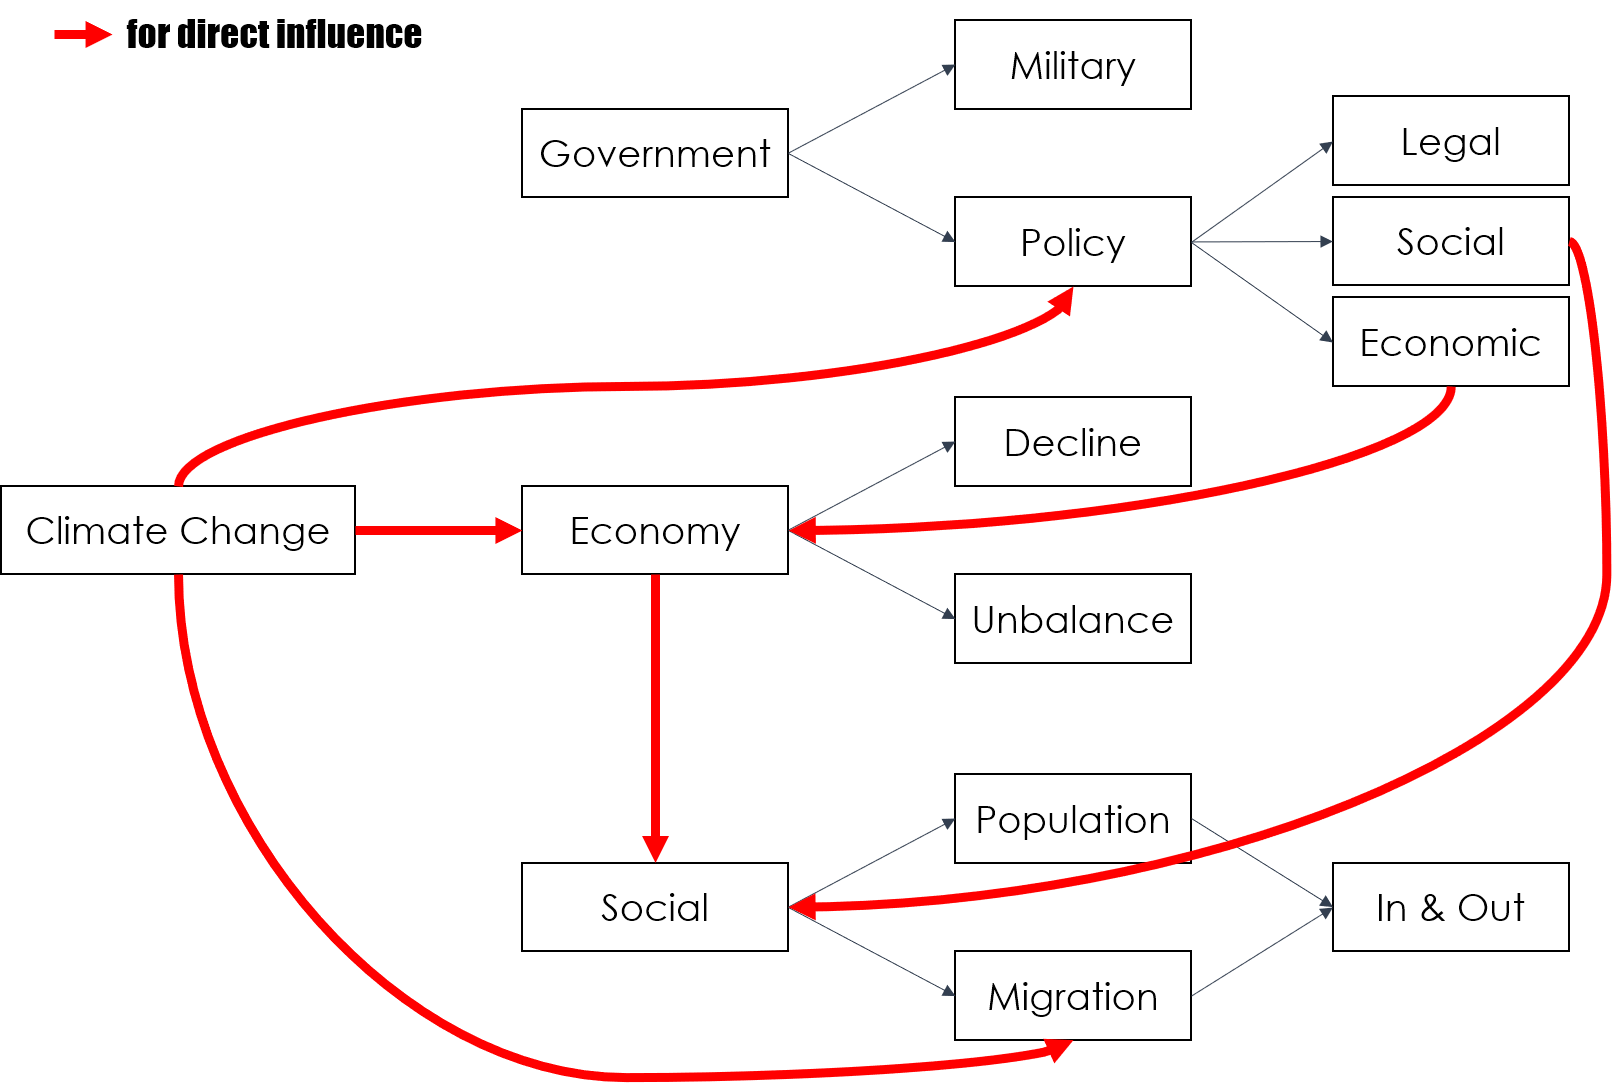
\includegraphics[width=14cm]{figure2.png}
		\caption{Stage-structured model of current process} \label{fig:Stage-structured model of current process}
	\end{figure}
	
	\noindent Additionally, the quantities involved in the function are shown in \textbf{Table 1} and \textbf{Table 2}. We list subscripts and primary notations apart.\\
	
	\begin{table}[htbp]
		\renewcommand\arraystretch{1.5}
		\footnotesize
		\centering
		\begin{tabular}{m{3cm}<{\centering}|m{10cm}<{\centering}}
			\whline
			\textbf{Subscript}&\textbf{Definition}\\
			\whline 
			$N$&$N_{th}$ year\\ 
			\shline
		\end{tabular}
		\caption{Definition of Subscripts in the model}\label{tab:Definition of Subscripts in the model}
	\end{table}
	\begin{table}[htbp]
		\renewcommand\arraystretch{1.5}
		\footnotesize
		\centering
		\begin{tabular}{m{3cm}<{\centering}|m{10cm}<{\centering}}
			\whline
			\textbf{Notation}&\textbf{Definition}\\
			\whline 
			$F$&Degree of Fragility\\
			$C$&Climate factor\\
			$E$&Economic factor\\
			$S$&Social factor\\
			$P$&Policy factor\\ 
			$M$&Military factor\\
			$X$&External Intervention\\
			\shline
		\end{tabular}
		\caption{Definition of notations in the model}\label{tab:Definition of notations in the model}
	\end{table}
	
	To evaluate the fragility of a country, we define the evaluation function $F$
	
	\begin{equation}
	F_N = w 
	\left(
	\begin{matrix}
	P_N \\ M_N \\ E_N \\ S_N
	\end{matrix}
	\right)
	\end{equation}
	
	In the function, $w$ is the weight of the variables, which is $(w_1, w_2, w_3, w_4)$. Since in the subsequent paragraphs we will normalize $P_N, M_N, E_N, S_N$, and for conciseness of the formula, we could assign w to be 1 for each variable.
	
	As assumed, if climate and external intervention remains zero, our major factors should be a \textbf{Markov Model}, which is
	
	$$
	\left(
	\begin{matrix}
	P_{N+1} \\ M_{N+1} \\ E_{N+1} \\ S_{N+1}
	\end{matrix}
	\right) 
	= 
	\left(
	\begin{matrix}
	k_{11} & k_{12} & k_{13} & k_{14} \\
	k_{21} & k_{22} & k_{23} & k_{24} \\
	k_{31} & k_{32} & k_{33} & k_{34} \\
	k_{41} & k_{42} & k_{43} & k_{44} \\
	\end{matrix}
	\right) 
	\left(
	\begin{matrix}
	P_N \\ M_N \\ E_N \\ S_N
	\end{matrix}
	\right) 
	$$
	Specifically, $P$ is the negative effect of improper policy issued by the government, $M$ is the decrease of security apparatus, $E$ is economic declining, and $S$ is social unrest. Assume coefficient matrix is $K$, then the function becomes
	$$
	\left(
	\begin{matrix}
	P_{N+1} \\ M_{N+1} \\ E_{N+1} \\ S_{N+1}
	\end{matrix}
	\right) 
	= 
	K
	\left(
	\begin{matrix}
	P_N \\ M_N \\ E_N \\ S_N
	\end{matrix}
	\right) 
	$$
	
	\subsection{Modified Markov Model including climate change}
	
	We can find in the schema (\textbf{Figure 1}) that climate change has direct influence on \textbf{policy factor}, \textbf{economy factor} and \textbf{social factor}, which indicates that there are several modifications to make. Since only the \textbf{military factor} is not affected, the modified prediction function should be as follow
	
	$$
	\left(
	\begin{matrix}
	P_{N+1} \\ M_{N+1} \\ E_{N+1} \\ S_{N+1}
	\end{matrix}
	\right) 
	= 
	K 
	\left(
	\begin{matrix}
	P_N \\ M_N \\ E_N \\ S_N
	\end{matrix}
	\right) 
	+
	K_c
	C
	+ X
	, \quad
	K_c = 
	\left(
	\begin{matrix}
	k_{CP} \\ {0} \\ k_{CE} \\ k_{CS}
	\end{matrix}
	\right)
	$$
	$P_{CP},P_{CE}$ and $P_{CS}$ are the influence of climate change on policy, economic and social factors. $X$ is external intervention, and here we assume it to be 0. There may be doubts whether \textbf{military factor} will be affected. As a matter of fact, \textbf{military factor} will change, but not on the direct effect of climate change. The indirect influence from climate change will appear while running the modified prediction function. For example, catastrophe causes social instability, then the military level changes, which might take some time for strategic planning.
	
	
	\subsection{Estimation for some parameters}
	
	We apply quantitative analysis on the influence of climate change (\textbf{Table 3}) and interplay of other factors (\textbf{Table 4}). The figures in each cell denote the number of studies that support, do not support, or contradict the proposed hypothesis. 
	\begin{table}[htbp]
		\renewcommand\arraystretch{1.5}
		\footnotesize
		\centering
		\begin{tabular}{m{3.8cm}<{\centering}|m{4.8cm}<{\centering}|m{4.8cm}<{\centering}}
			\whline
			\textbf{Hypothesis}&\textbf{$P_N$}&\textbf{$M_N$}\\
			\whline
			\textbf{Abnormal precipitation}& 2 support, 1 none, 1 opposite &1 support, 2 none, 1 opposite\\
			
			\textbf{Abnormal temperature}&1 support, 2 none, 1 opposite&1 support, 1 none, 1 opposite\\
			
			\textbf{Natural disasters}&2 support, 1 opposite&1 none\\
			
			\textbf{Sea level rising}&2 support, 1 none, 1 opposite&1 support, 1 none, 1 opposite\\
			
			\textbf{Energy deficiency}&2 support, 1 opposite&3 none\\
			
			\textbf{Less vegetation}&2 none&1 none\\
			
			\shline
			\textbf{Hypothesis}&\textbf{$E_N$}&\textbf{$S_N$}\\
			\whline
			\textbf{Abnormal precipitation}& 3 support, 1 some support &2 support, 1 opposite\\
			
			\textbf{Abnormal temperature}&4 support, 1 none, 2 opposite&2 support, 1 none, 1 opposite\\
			
			\textbf{Natural disasters}&6 support, 1 opposite&6 support, 2 opposite\\
			
			\textbf{Sea level rising}&3 support, 1 none, 1 opposite&2 none\\
			
			\textbf{Energy deficiency}&2 support, 1 opposite&2 support, 1 none, 1 opposite\\
			
			\textbf{Less vegetation}&3 support, 1 none, 1 opposite&2 support, 1 opposite\\
			\shline
		\end{tabular}
		\caption{Influence of climate change - Quantitative study}\label{tab:Influence of climate change - Quantitative study}
	\end{table}
	
	\begin{table}[htbp]
		\renewcommand\arraystretch{1.5}
		\footnotesize
		\centering
		\begin{tabular}{m{2.7cm}<{\centering}|m{5cm}<{\centering}|m{5cm}<{\centering}}
			\whline
			\textbf{Hypothesis}&\textbf{$P_N$}&\textbf{$M_N$}\\
			\whline
			\textbf{$P_N$}&3 support &2 support, 1 none, 2 opposite\\
			
			\textbf{$M_N$}&2 support, 1 none, 2 opposite&4 support\\
			
			\textbf{$E_N$}&4 support, 1 none&1 support, 1 opposite\\
			
			\textbf{$S_N$}&1 support, 1 none&2 support, 1 none, 1 opposite\\
			\shline
			\textbf{Hypothesis}&\textbf{$E_N$}&\textbf{$S_N$}\\
			\whline
			\textbf{$P_N$}& 3 support, 1 none, 1 opposite & 1 support, 1 none\\
			
			\textbf{$M_N$}&1 support, 2 none&1 support, 1 none\\
			
			\textbf{$E_N$}&3 support&1 support, 2 none\\
			
			\textbf{$S_N$}&1 support, 2 none&1 support\\
			\shline
		\end{tabular}
		\caption{Interplay of different factors - Quantitative study}\label{tab:Interplay of different factors - Quantitative study}
	\end{table}
	The total number of reviewed studies per outcome is computed and will be used for the computation of parameters. To be more specific, for each cell we need to calculate an parameter that represents the influence of the row factor on the column factor. If there is a study that supports the relation, we increase the outcome by 1; if there is a study that is opposite to the relation, we decrease it by 1. Then we calculates the sum of each row, and consider the proportion of each cell in the sum as the parameter of that cell. 
	
	Finally ,we attain matrix $K$ and $K_c$ as follows
	\begin{spacing}{1.5}
		$$
		K = 
		\left(
		\begin{matrix}
		\frac{1}{2} & 0 & \frac{1}{3} & \frac{1}{6} \\
		0 & \frac{2}{3} & \frac{1}{6} & \frac{1}{6} \\
		\frac{1}{2} & 0 & \frac{3}{8} & \frac{1}{8} \\
		\frac{1}{4} &\frac{1}{4} & \frac{1}{4} & \frac{1}{4} \\
		\end{matrix}
		\right) 
		, \quad K_c = 
		\left(
		\begin{matrix}
		\frac{1}{8} \\ {0} \\ \frac{1}{2} \\ \frac{1}{4}
		\end{matrix}
		\right) 
		$$
	\end{spacing}
	Therefore, the final prediction function becomes
	\begin{spacing}{1.5}
		\begin{equation}
		\left(
		\begin{matrix}
		P_{N+1} \\ M_{N+1} \\ E_{N+1} \\ S_{N+1}
		\end{matrix}
		\right) 
		= 
		\left(
		\begin{matrix}
		\frac{1}{2} & 0 & \frac{1}{3} & \frac{1}{6} \\
		0 & \frac{2}{3} & \frac{1}{6} & \frac{1}{6} \\
		\frac{1}{2} & 0 & \frac{3}{8} & \frac{1}{8} \\
		\frac{1}{4} &\frac{1}{4} & \frac{1}{4} & \frac{1}{4} \\
		\end{matrix}
		\right) 
		\left(
		\begin{matrix}
		P_N \\ M_N \\ E_N \\ S_N
		\end{matrix}
		\right) 
		+
		\left(
		\begin{matrix}
		\frac{1}{8} \\ {0} \\ \frac{1}{2} \\ \frac{1}{4}
		\end{matrix}
		\right) 
		C
		+ X
		\end{equation}
	\end{spacing}	
	
	\subsection{Obtain fragility standard}
	It makes no sense to draw up standards out of an imaginary country, so we choose to investigate several countries which are widely accepted as stable, vulnerable and fragile.
	We respectively define Egypt, China and Italy to be fragile, vulnerable and stable, then we do research in Fragile States Index database[3] to calculate the policy factor, military factor, economy factor and social factor. Our factors are gained by 
	\begin{spacing}{1.5}
		\begin{equation}
		\begin{aligned}
		&P=\frac{1}{2}PS+\frac{1}{2}HR\\
		&M=SA\\
		&E=\frac{1}{3}EC+\frac{1}{3}UD+\frac{1}{3}HF\\
		&S=\frac{1}{2}DP+\frac{1}{2}RI\\
		\end{aligned}
		\end{equation}
	\end{spacing}
	
	The results are as follows (\textbf{Table 5})
	
	\begin{table}[htbp]
		\renewcommand\arraystretch{1.5}
		\footnotesize
		\centering
		\begin{tabular}{m{2cm}<{\centering}|m{2cm}<{\centering}|m{2cm}<{\centering}|m{2cm}<{\centering}|m{2cm}<{\centering}}
			\whline
			&\textbf{$P$}&\textbf{$M$}&\textbf{$E$}&\textbf{$S$}\\
			\whline
			\textbf{Italy}& 2.35 & 4.5 & 3.43 & 4.9\\
			
			\textbf{China}& 7.1 & 5.9 & 5.53 & 5.8\\
			
			\textbf{Egypt}& 7.35 & 8.1 & 6.3 & 7.2\\
			
			\shline
		\end{tabular}
		\caption{Factors of Italy, China and Egypt}\label{tab:Factors of Italy, China and Egypt}
	\end{table}
	After getting these data, we use the evaluation function $(1)$ to obtain their fragility. (\textbf{Table 6})
	
	\begin{table}[htbp]
		\renewcommand\arraystretch{1.5}
		\footnotesize
		\centering
		\begin{tabular}{m{2cm}<{\centering}|m{5cm}<{\centering}}
			\whline
			&\textbf{$F$}\\
			\whline
			\textbf{Italy} & 15.1833\\
			
			\textbf{China} & 24.33\\
			
			\textbf{Egypt} & 28.95\\
			
			\shline
		\end{tabular}
		\caption{Fragility of Italy, China and Egypt}\label{tab:Fragility  of Italy, China and Egypt}
	\end{table}
	
	So we can now define stable as fragility below 15.18, vulnerable as fragility above 24.33 and fragile as fragility above 28.95.
	
	\subsection{The Impact of Climate Change}
	
	In this section, we use an example to further illustrate the impact of climate change. Applying our model, we measure the impact of climate change and analyze how it changes the fragility of a state. We first assume the change of climate is random, and compare the fragility of the country with and without the influence of climate change. Then we assume the climate change is always negative, and do the same comparison.
	
	As is shown in \textbf{Figure 2},  calculated by our model above, the red line represents the fragility of the country as time passes without the influence of climate change; the green line is the fragility with the indirect influence of climate change; the blue line is the fragility with the indirect and direct influence of climate change. According to the figure, the impact of climate change has both positive and negative side. 
	\begin{figure}[h]
		\small
		\centering
		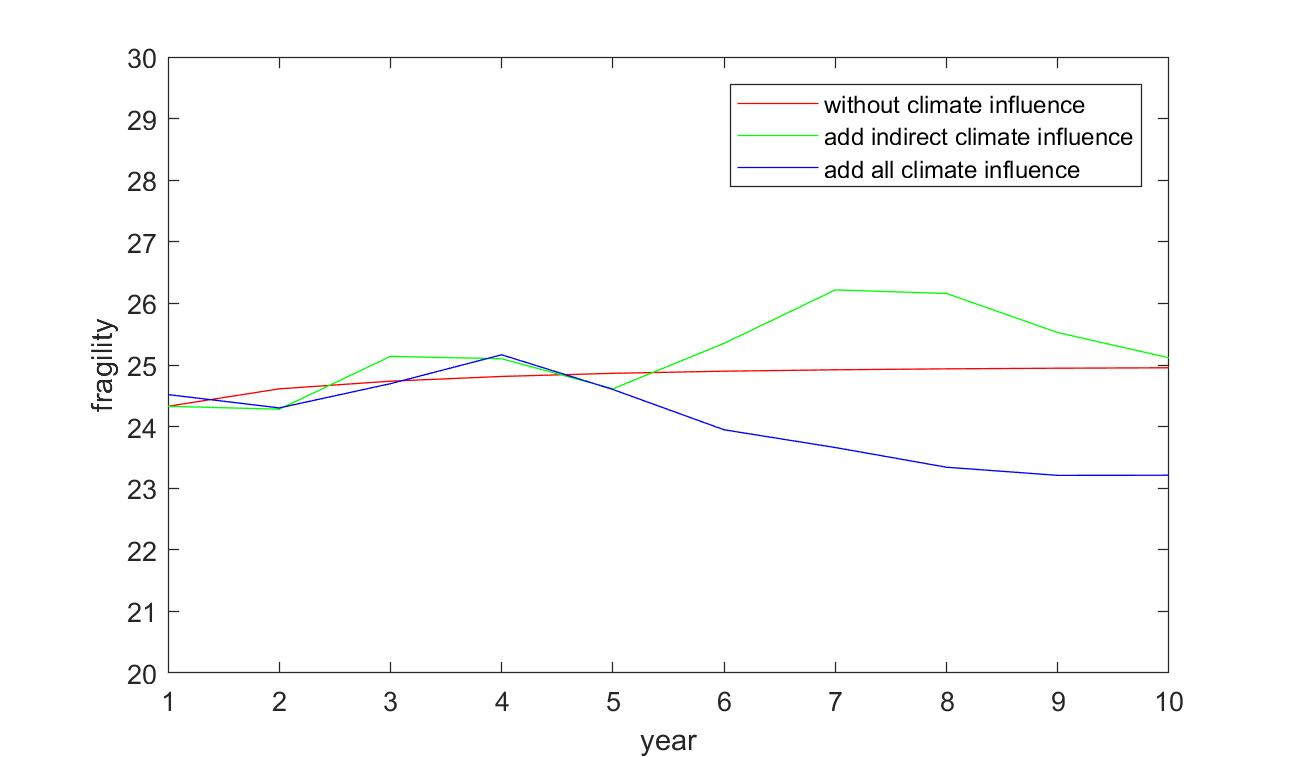
\includegraphics[width=12cm]{figure3.jpg}
		\caption{Fragility-Year Graph with random climate change} \label{fig:Fragility-Year with random climate change}
	\end{figure}

	In \textbf{Figure 3}, the implication of each line is same as what is illustrated above. It is clear that climate change increases fragility of the country. It will cause such consequence through direct impact and indirect means, which accords with the discussion in the previous chapters.
	\begin{figure}[h]
		\small
		\centering
		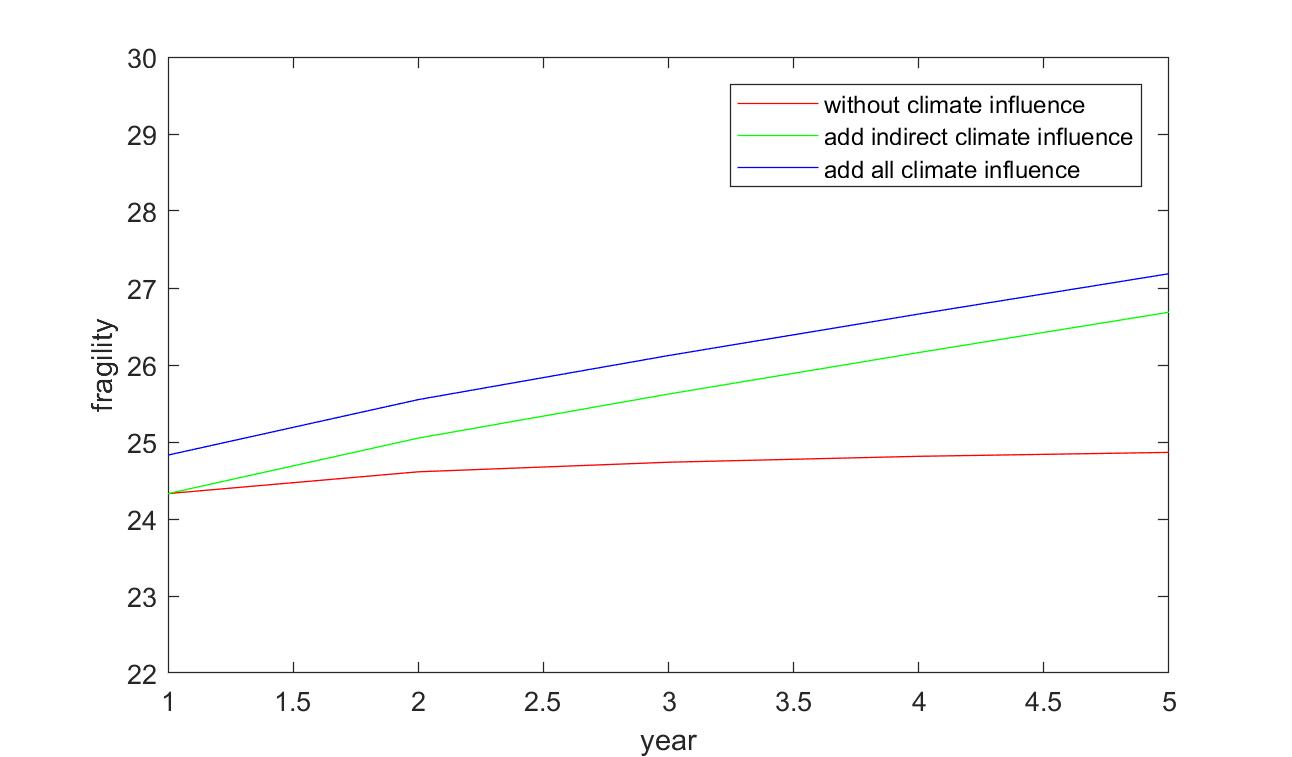
\includegraphics[width=12cm]{figure4.jpg}
		\caption{Fragility-Year Graph with negative climate change} \label{fig:Fragility-Year with random climate change}
	\end{figure}
	
	\section{Run model on the most fragile country}
	\subsection{How climate change increase fragility}
	In the section above, we have already build up our evaluation model of fragility. To test this model on some extreme situation, we first select one of the most fragile country: Central African Republic, which is on the edge of crashing. Its basic information are shown in \textbf{Table 7}

	\begin{table}[htbp]
		\renewcommand\arraystretch{1.5}
		\footnotesize
		\centering
		\begin{tabular}{m{2.5cm}<{\centering}|m{2.5cm}<{\centering}|m{2.5cm}<{\centering}|m{2.5cm}<{\centering}|m{2.5cm}<{\centering}}
			\whline
			\textbf{C1: Security Apparatus}&\textbf{C2: Factionalized Elites}&\textbf{C3: Group Grievance}&\textbf{E1: Economy}&\textbf{E2: Economic Inequality} \\
			\whline
			9.0 & 9.7 & 9.1 & 9.1 & 10.0\\
			\whline
			\textbf{E3: Human Flight and Brain Drain}&\textbf{P1: State Legitimacy}&\textbf{P2: Public Services}&\textbf{P3: Human Rights}&\textbf{S1: Demographic Pressures} \\
			\whline
			7.5 & 9.7 & 10.0 & 9.7 & 9.0\\
			\whline
			\textbf{S2: Refugees and IDPs}&\textbf{X1: External Intervention}&\textbf{Total}& \textbf{Rank} & \\
			\whline
			10.0 & 9.8 & 112.6 & 3rd &\\
			\shline
		\end{tabular}
		\caption{Info of Central African Republic in 2017}\label{tab:Info of Central African Republic in 2017}
	\end{table}
	
	
	In the Fragile States Index database, we can find some major factors for our model. After data conversion, we obtain the inputs for our prediction function (\textbf{Table 8})
	
	\begin{table}[htbp]
		\renewcommand\arraystretch{1.5}
		\footnotesize
		\centering
		\begin{tabular}{m{2.5cm}<{\centering}|m{2.5cm}<{\centering}|m{2.5cm}<{\centering}|m{2.5cm}<{\centering}}
			\whline
			\textbf{$P$}&\textbf{$M$}&\textbf{$E$}&\textbf{$S$}\\
			\whline
			9.85 & 9 & 8.87 & 9.5 \\
			\shline
		\end{tabular}
		\caption{Factors of Central African Republic}\label{tab:Factors of Central African Republic}
	\end{table}
	
	First, we want to determine how climate change may have increased fragility of Central African Republic, which is similar to what we have done in the last section. We assume the climate change to be a constant negative factor. The fragility of Central African Republic in 5 years is shown in \textbf{Figure 4}
	
	\begin{figure}[h]
		\small
		\centering
		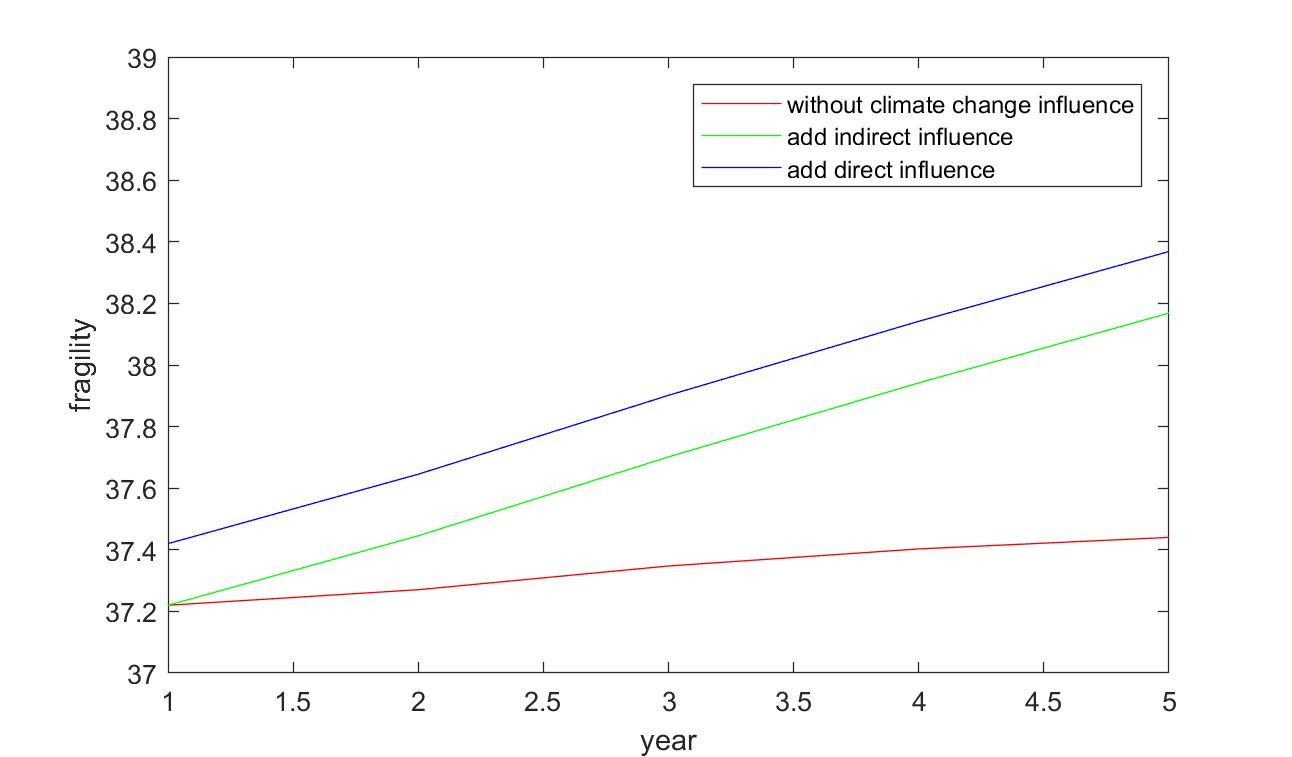
\includegraphics[width=12cm]{figure5.jpg}
		\caption{Fragility-Year Graph of Central African Republic} \label{fig:Fragility-Year Central African Republic}
	\end{figure}
	
	It is apparent that if climate continue to be negative, a country will find it hard to adjust its policy, economy and society to reduce fragility. The fragility of Central African Republic is high enough in 2017, which can be even worse if climate remains harmful.


	\subsection{Ways to mitigate fragility}
	Then we try to find the fragility trend without climate change factor. Among the four factors we defined, policy factor is the only one that government can control, others can only be affected by the policy factor. So, we set climate factor to 0 and change policy factor, trying to find the value of policy factor when fragility won’t get worse in 5 years.
	
	\textbf{Figure 5} is the fragility changing curve when policy factor is down to 9.37, the fragility will get better in 2 years then adjust itself to become as fragile as before, which indicate that in this kind of country, positive policy may not last long in current situation.
	
	\begin{figure}[h]
		\small
		\centering
		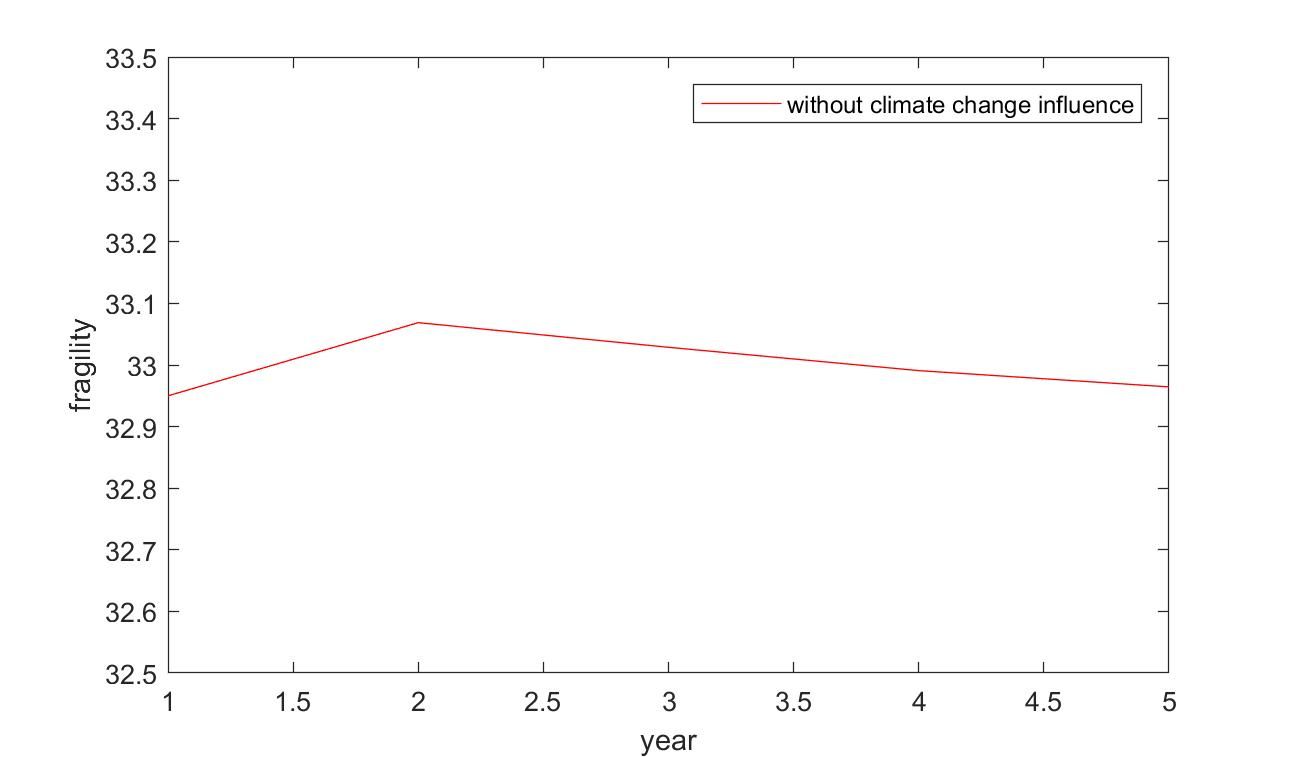
\includegraphics[width=12cm]{figure6.jpg}
		\caption{Fragility-Year of Graph Central African Republic} \label{fig:Fragility-Year Central African Republic}
	\end{figure}
	
	So, the conclusion can be drawn: If government can still make right, positive decisions on economic and social policies, then the fragility might not get higher. If this country wants to be less fragile, its government should be very capable and outstanding on making right decisions, which might not be the case in most fragile countries.

	\section{Run model on the stable country}
	\subsection{Refine model with more specific climate change}
	In this chapter, we choose countries with high stability for data analysis, since such countries have dramatic difference with countries involved in the previous discussion. Furthermore, the choice of country will affect our choice of climate parameters. For example, if we choose landlocked countries, the impact of sea-level rise should not be a major factor.
	
	Select a specific N as iteration time. Assume each climate factor is $C_i$, and the corresponding weight is $k_{c_i}$.  We iterate under the constraint condition that the fragility of a state does not increase ($F_0 = F_N$). Therefore, we have the following equation
	
	$$
	\Sigma k_{c_i} C_i \leq const
	$$
	
	The weight assigned to each factor reflects the degree of influence of the corresponding climate factor on the fragility of a country.
	
	In practice, we select the Netherlands to calculate the impact of the climate. After researching on the national conditions in the Netherlands, we find that climate factors that have a major impact on the fragility of the Netherlands include: anomalies in temperature ($T$), anomalies in rainfall ($R$), sea-level rise ($L$) and natural disasters ($D$), which have significant influence on policy, military, economic and social factors. After assigning proper weights, we can write the influence matrix and the vector of climate factor as follows:
	\begin{spacing}{1.5}
	$$
	\left(
	\begin{matrix}
	P_{N+1} \\ M_{N+1} \\ E_{N+1} \\ S_{N+1}
	\end{matrix}
	\right) 
	= 
	K 
	\left(
	\begin{matrix}
	P_N \\ M_N \\ E_N \\ S_N
	\end{matrix}
	\right) 
	+
	K_c
	\left(
	\begin{matrix}
	T \\ R \\ L \\ D \\
	\end{matrix}
	\right)
	+ X
	, \quad
	K_c = 
	\left(
	\begin{matrix}
		\frac{1}{8} & \frac{1}{4} & \frac{1}{8} & \frac{1}{2} \\
		0 & \frac{1}{4} & 0 & \frac{3}{4} \\
		\frac{1}{4} & \frac{1}{4} & \frac{1}{4} & \frac{1}{4} \\
		\frac{1}{3} & \frac{1}{3} & 0 & \frac{1}{3} \\
	\end{matrix}
	\right)
	$$
	\end{spacing}

	\subsection{Run model on the Netherlands}
	We select $N = 5$ as iteration time, and attain the equation that could satisfy the constrain condition:
	$$
	8.96D + 0.22E + 2.24L - 0.41M + 0.52P + 5.31R - 0.33S + 3.49T\leq0
	$$
	After assigning the data of the Netherlands in Fragile States Index database, we can attain
	$$
	8.96D + 2.24L + 5.31R + 3.49T - 0.58\leq0
	$$
	Figures of this equation are shown in \textbf{Figure 6}. From the figures, we can observe the relations between $D,T,R,L$ clearly and intuitively.
	
	\begin{figure}[h]
		\small
		\centering
		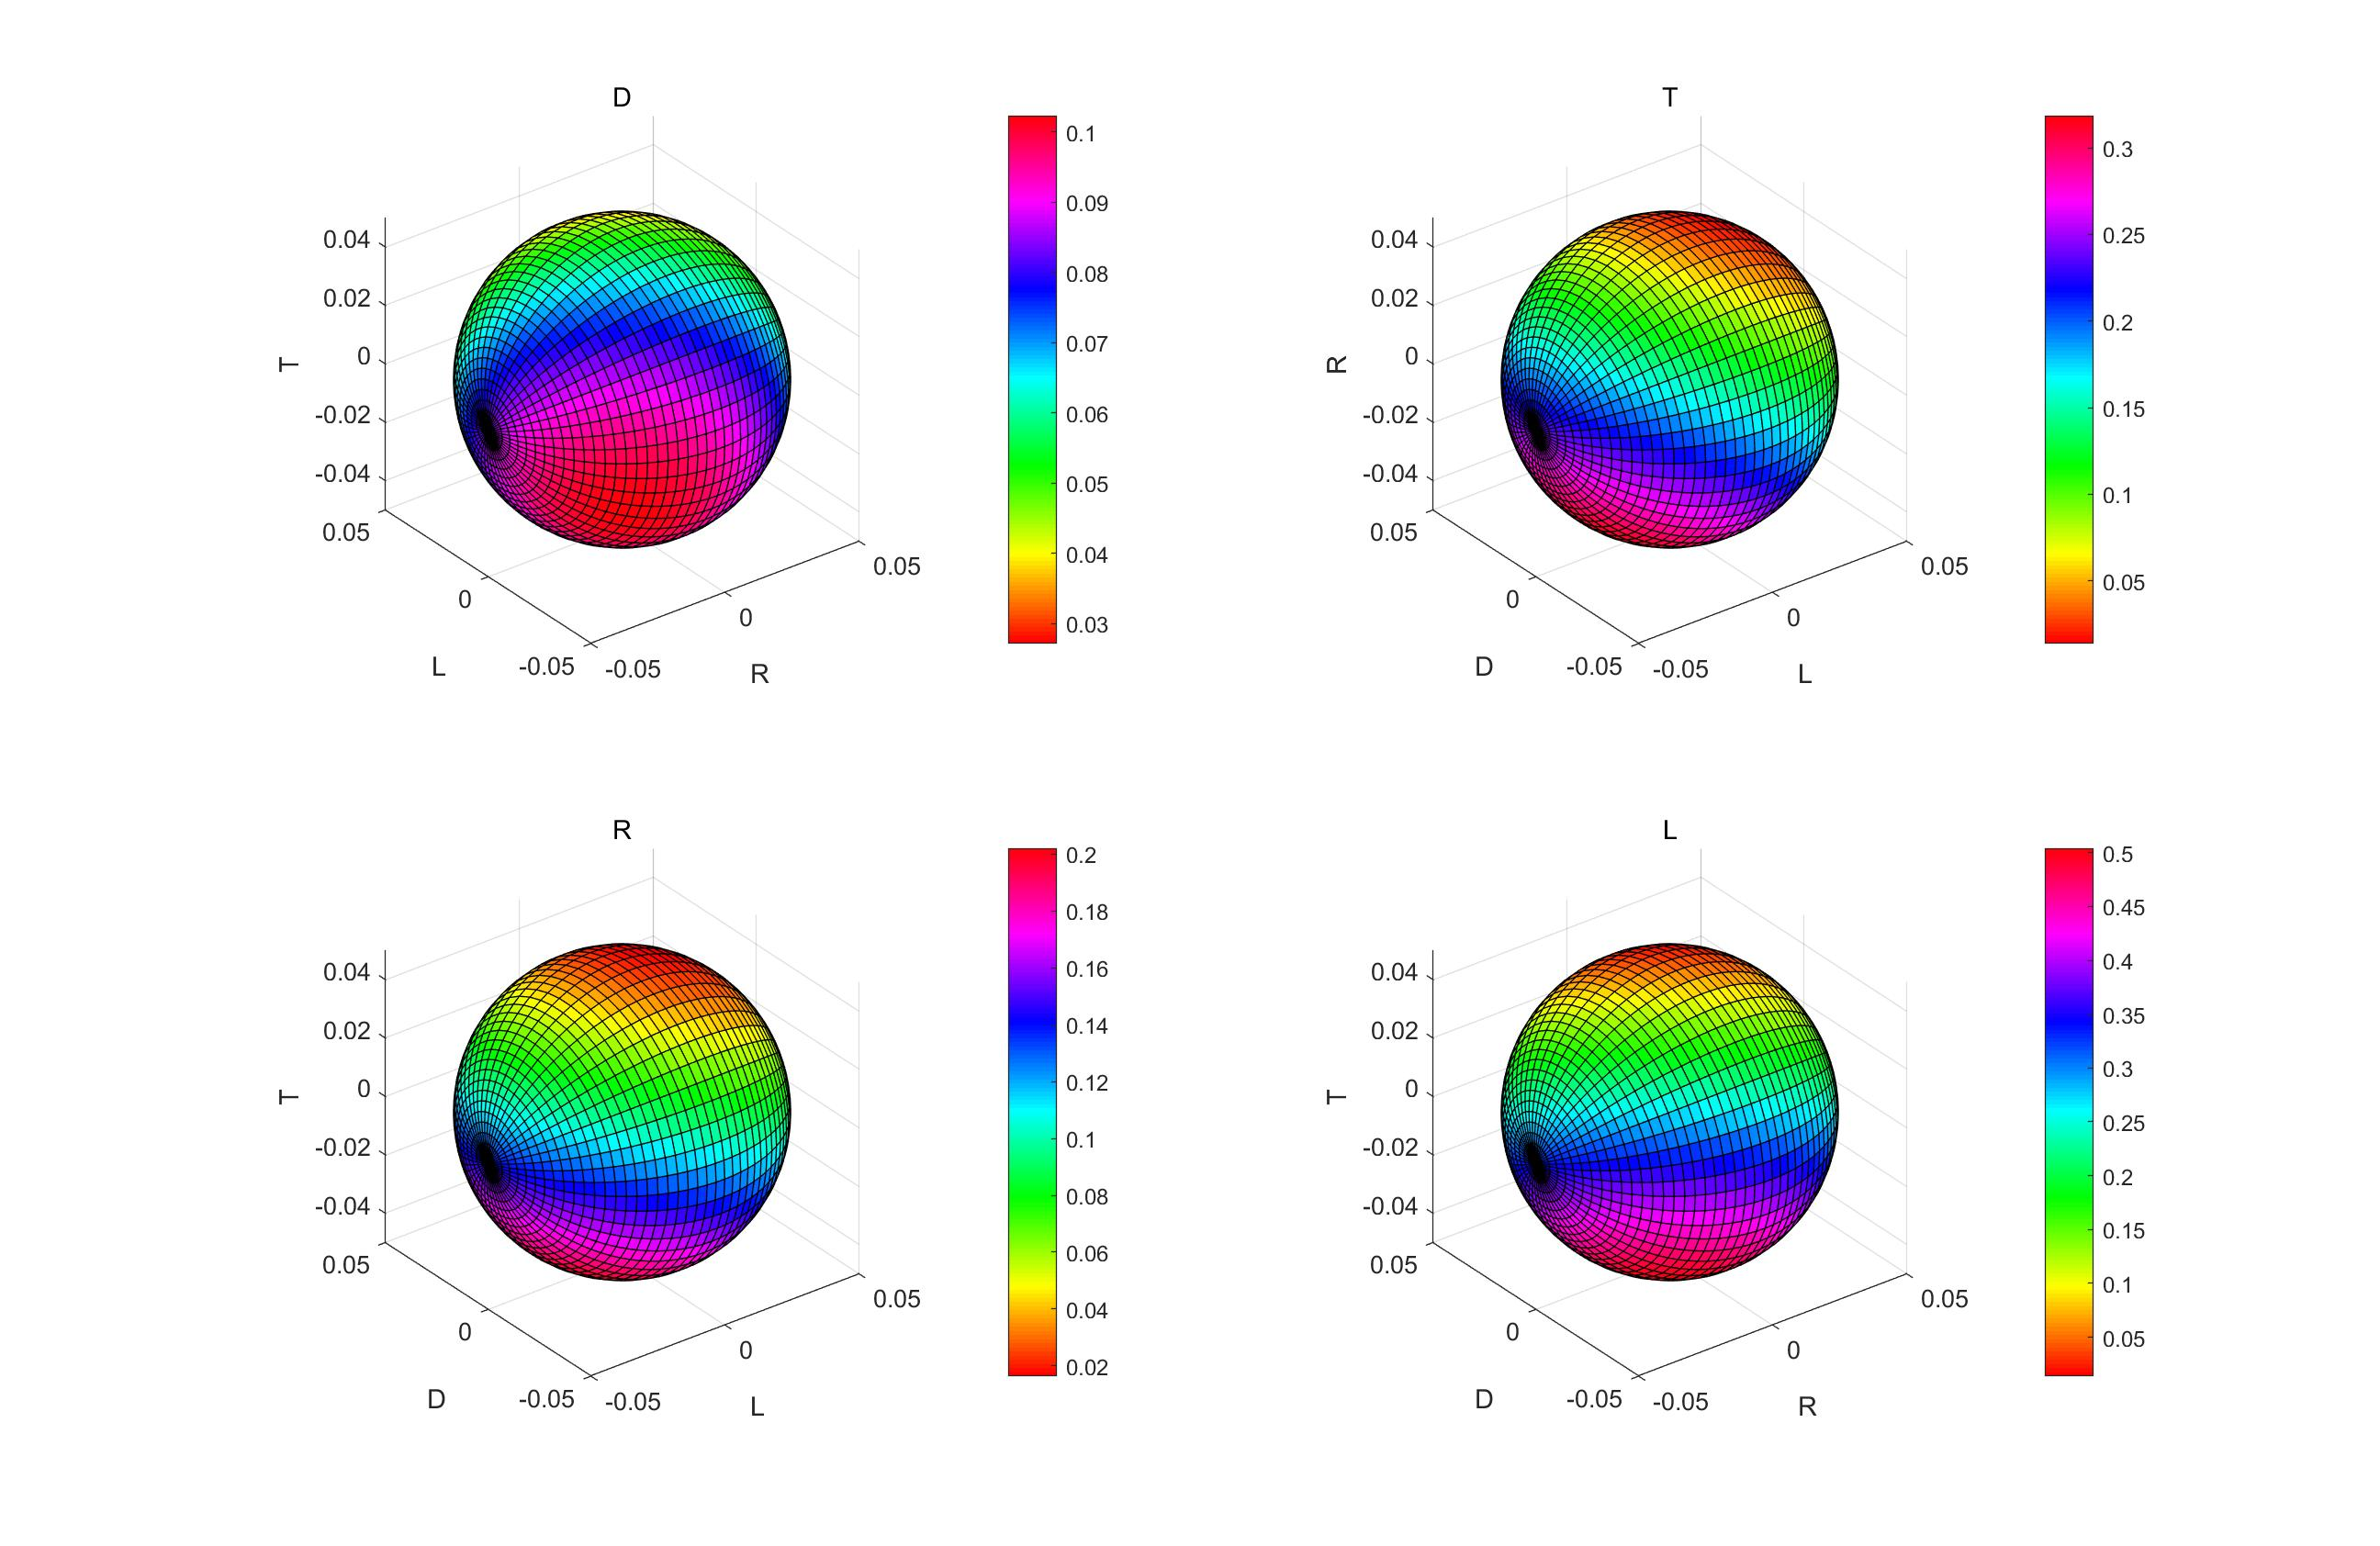
\includegraphics[width=16cm]{figure7.jpg}
		\caption{Figure of Climate Equation} \label{fig:Figure of Climate Equation}
	\end{figure}
	
	When the equation cannot be satisfied, which means the impact of climate change goes beyond the capacity of the Netherlands to regulate and control, the Netherlands will become more fragile within five years.
	The tipping point is when the climate change in the Netherlands satisfies
	$$
	8.96D + 2.24L + 5.31R + 3.49T - 0.58 = 0
	$$
	
	
	It can be seen that these climate factors have different effects on whether the equation can be satisfied, according to their coefficients in the equation. Natural disasters have the greatest influence. In another word, it is really difficult to completely avoid loss through various policies when serious natural disasters occur. In addition,  the sea-level rise has relatively less impact on the Netherlands. In practice, however, natural disasters in the Netherlands occur less frequently, while sea-level rise is a constant threat to the Netherlands due to the low elevation and can easily affect social stability by causing massive immigration and declining social order. So if we want to get a universal and complete evaluation of a country, we also need to investigate the various climate factors in the country and the frequency and duration of their occurrence.
	
	\section{Impact of Driven Interventions on Fragility}
	\subsection{Refine the Model}
	In this chapter, we continue to use the Netherlands as an example to build our model. Impact of major climate factors in the Netherlands, which are Anomalies in temperature ($T$), anomalies in rainfall ($R$), sea-level rise ($L$) and natural disasters ($D$) can all be remedied through specific policies. If the government investment in coping with climate change is not sufficient, climate change will cause an enormous influence on the fragility of the country; however, if government invest too much in it, economy of the country could be affected. We should find a tradeoff between cost of policies and impact of climate change. 
	
	According to four major climate factors, we mainly enumerate four policies, or driven interventions, to mitigate the risk of climate change. Interventions include artificial rainfall and building reservoirs ($P_w$), air conditioning subsidies ($P_a$), building dams ($P_d$), and monitoring and early warning of natural disasters ($P_m$). \textbf{Figure }
	
	\begin{figure}[h]
		\small
		\centering
		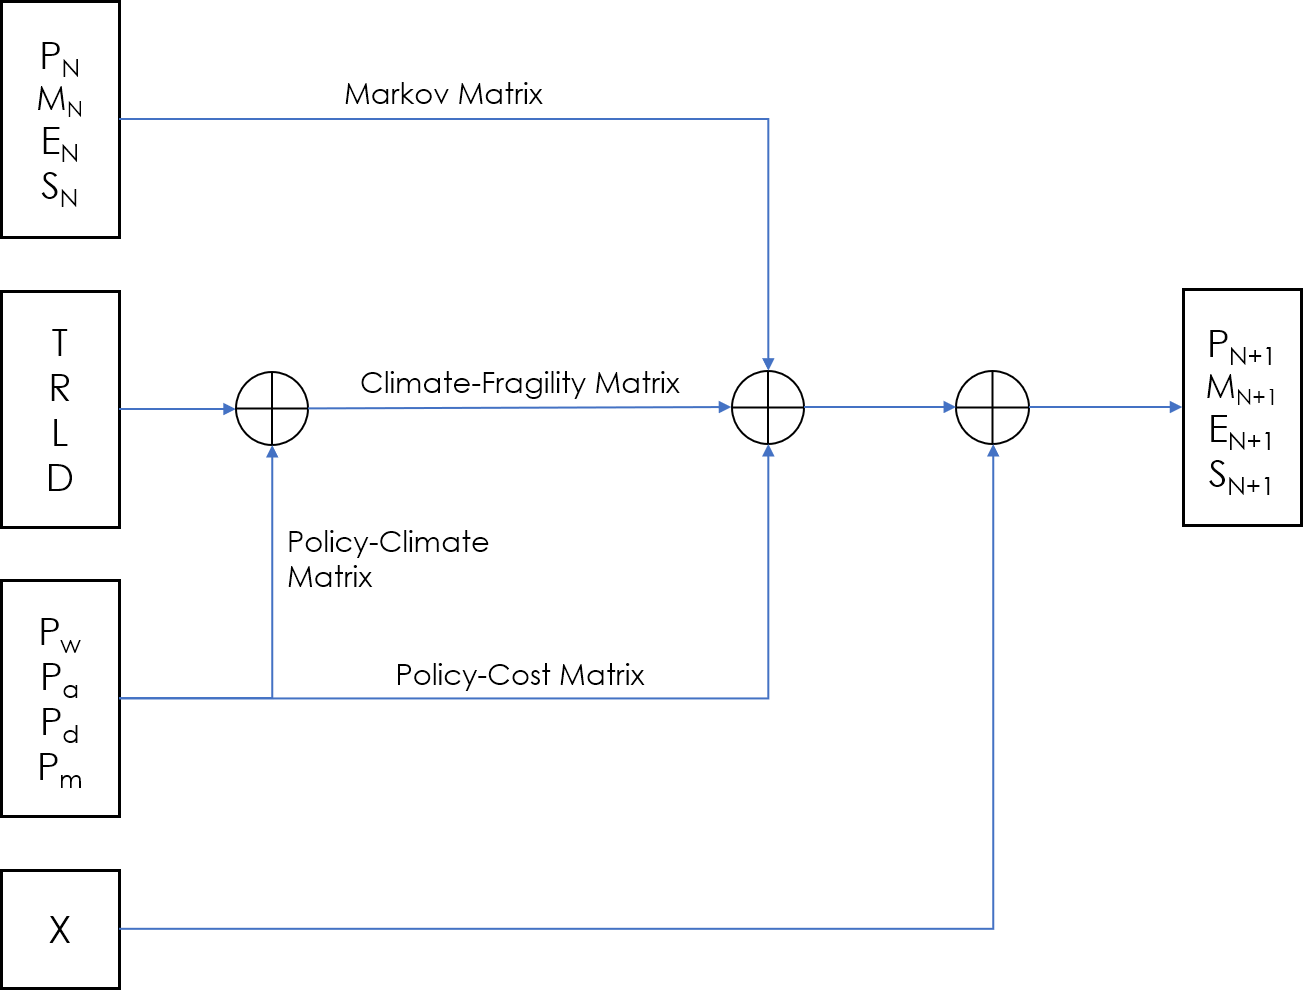
\includegraphics[width=15cm]{figure8.png}
		\caption{Schema of refined model} \label{fig:Schema of refined model}
	\end{figure}
	
	From what have been discussed, we modify our model as follows
	  	\begin{spacing}{1.5}
	  	$$
	  	\left(
	  	\begin{matrix}
	  	P_{N+1} \\ M_{N+1} \\ E_{N+1} \\ S_{N+1}
	  	\end{matrix}
	  	\right) 
	  	= 
	  	K 
	  	\left(
	  	\begin{matrix}
	  	P_N \\ M_N \\ E_N \\ S_N
	  	\end{matrix}
	  	\right) 
	  	+
	  	K_c
	  	\left(
	  	\left(
	  	\begin{matrix}
	  	T \\ R \\ L \\ D \\
	  	\end{matrix}
	  	\right)
	  	+ 
	  	K_p
	  	\left(
	  	\begin{matrix}
	  	P_w \\ P_a \\ P_d \\ P_m \\
	  	\end{matrix}
	  	\right)
	  	\right)
	  	+
	  	K_{pc}
	  	\left(
	  	\begin{matrix}
	  	P_w \\ P_a \\ P_d \\ P_m \\
	  	\end{matrix}
	  	\right)
	  	+ X
	  	$$
	  \end{spacing}
	This function includes the effect of interventions on both climate change and country's economy. $K_p (P_w, P_a, P_d, P_m)^T$ is the effect of interventions on climate change, and $K_{pc} (P_w, P_a, P_d, P_m)^T$ is the cost of the interventions, which influences economy.
	
	\subsection{Estimation for Parameters and Calculation of Model}
	In order to make the model clear, we use the capital investment required to implement the policy as the input for this policy, which means $P_w, P_a, P_d, P_m$ are cost of each policy, so $K_{pc}$ can be written as below
	$$
	K_{pc} = 
	\left(
	\begin{matrix}
		0 & 0 & 0 & 0 \\
		0 & 0 & 0 & 0 \\
		1 & 1 & 1 & 1 \\
		0 & 0 & 0 & 0 \\
	\end{matrix}
	\right)
	$$
	We estimate each policy's effect on alleviating the risk of climate change with the same cost. So we can attain $K_p$ as follows
	\begin{spacing}{1.5}
		$$
		K_{pc}=
		\left(
		\begin{matrix}
		-\frac{1}{3} & -\frac{2}{3} & 0 & 0 \\
		-1 & 0 & 0 & 0 \\
		0 & 0 & -1 & 0 \\
		-\frac{1}{6} & -\frac{1}{6} & -\frac{1}{6} & -\frac{1}{2} \\
		\end{matrix}
		\right)
		$$
	\end{spacing}
	As the impact of human intervention policies is usually short, we reduce the iteration time to one year. The iteration result is
	$$
	1.833D + 0.125E + 0.375L - 0.083M + 0.250P + 1.083R - 0.292S 
	$$
	$$
	 + 0.708T + 0.222Pa + 0.319Pd + 0.083Pm - 0.625Pw \leq 0
	$$
	Similar to the previous analysis, if the equation above is satisfied, the fragility of the state will not be increased, which means such interventions can prevent a country from becoming a fragile state.
	
	We use data of the Netherlands in 2017 from Fragile States Index database to calculate, and obtain the following equation
	$$
	1.833D + 0.375L + 1.083R + 0.708T
	$$
	$$
	 + 0.222Pa + 0.319Pd + 0.083Pm - 0.625Pw \leq 0
	$$
	With the equation above, we can plan for the expenditure that the policy leads to. If we simply consider that we should not increase the fragility of a state, we should invest a larger proportion of the heavily weighted policies to minimize the total cost on the policies. In reality, more factors need to be considered. We can not ignore the impact of other climate factors. We should also invest enough funds for them.
	
	\subsection{Total Cost}
	The total cost of interventions for the country is the sum of $P_w, P_a, P_d$ and $P_m$.
	$$
	Cost = P_w + P_a + P_d + P_m
	$$
	What we give is a universal approach to calculate and predict the cost. However, the actual amount of the cost of each intervention depends on specific geographical location and local economic condition of the country, which means the cost of same policy may vary greatly in different country. Here we give a brief estimation of each policy based on the data accessible.
	
	Artificial rainfall using rockets is relatively cheap, and it requires rocket launchers and rockets. Each rocket launcher with towing trucks, need about 25,000\$, and each rocket needs about 400\$ as well as 200\$ for silver iodide flame shells. Transportation fees, escort fees, custodian fees and launch fees are also a huge cost of money. However, in addition to the equipment cost, weather conditions for making artificial rain need to be considered. In this case, it is necessary to launch a sounding balloon, and personnel should conduct data analysis on them. Therefore, an artificial rainfall needs about 30,000\$ - 50,000\$.
	
	Air conditioning subsidies relates to the population of the country. In China, each family may attain 30\$ to 60\$ per month.
	
	The cost of building dams includes cost of projects and facilities, and cost of land requisition and resettlement, which is greatly influenced by the local geography and geology conditions. According to the statistical analysis of the investment budget of several medium-sized dams in Chongqing, China, the total investment is estimated to be between 650,000\$ and 850,000\$, accounting for 70\% -35\% of the project costs and 30\% -65\% of the environmental costs of land acquisition and resettlement.
	
	Since different natural disasters requires different specialized monitoring and early warning system, the cost may be significantly different. Take earthquake as an example. According to the estimation from U.S. Geological Survey (USGS) in 2014, to build an earthquake early warning system covering the entire west coast of the United States, capital investment costs will reach 383,000,000\$ and annual maintenance and operational costs will be 161,000,000\$.
  
	\section{Analysis on universality of the model}
	\subsection{Smaller States}
	In the previous chapters, our model argues that external interventions have far less impact on policy, military, economic and social factors than domestic interventions. However, when the scope of the model is narrowed down to the size of a city, we think that the impact of external interventions will increase substantially and can not be ignored in the calculation. For example, when the earthquake disaster in a city usually receives the attention and help from the whole country, for a small state, the economic, policy and military aid input from the outside world can make up for the losses caused by the earthquake.
	
	In addition, we think the policy implementation in the smaller regions is more convenient and the weight of the influence of the policy will also increase, so the weight of the policy influence in the iteration matrix of the Markov model in chapter 3 should be increased.
	
	For a large country, there are more climate factors to consider. However, for a small city, there are often relatively stable climate factors. For example, in the earthquake-prone zone, more attention should be paid to the impact of natural disasters. Other factors such as temperature may be neglected.
	
	\subsection{Larger States}
	For larger regions, external inputs are usually smaller than individual countries and can therefore be ignored. Here we consider a certain continent to modify the model. The fragility of one continent should be affected by all the countries in the continent and the weights of influence of different countries are not the same. Countries with higher fragility have a greater impact on the fragility of the continent as a whole. For example, such countries may bring more local conflicts, refugees and other factors that increase fragility of the continent. So we use the root mean square of all countries in this continent to represent the fragility of the entire continent.
	$$
	F = \sqrt{\frac{\Sigma_{i=1}^n F_i^2}{n}}
	$$
	
	\section{Strengths and weaknesses}
	\begin{itemize}
		\item \large{\textbf{Strengths}}
		\begin{itemize}
			\item Our model separates the whole process of the variation of countries’ fragility into last year’s influence, climate change influence and external interventions, and independently analyzes every part of the model, which avoid the possible errors due to the complicated model.
			\item We use the logic of principal component analysis twice to divide the factors that affect the fragility of a country into five aspects: policy, economy, military, society and climate change. All the other factors will affect these five principal component factors. In addition, we divide the change of a country's climate into rainfall, temperature, sea level and natural disaster so as to make it clear and concise to evaluate the relationship between fragility of the country and the impact of climate change.
			\item The variation of countries’ fragility in every year is a discrete Markov process, so we abstract the process into a Markov chain model that simulates the variation of countries’ fragility and contributes to analyzing the relationship between fragility of the country and the impact of climate change.		
			\item In the specific analysis of the impacts of climate change on countries’ fragility, we select the Netherlands to do more comprehensive analysis. To be specific, we take the Netherlands's national conditions and geographical location, industrial structure, the relationship between the stability of the country and climate change in detail into consideration. Therefore, it has a good robustness.	
		\end{itemize}

		\item \large{\textbf{Weaknesses}}
			\begin{itemize}
				\item We use the Markov model to simulate the variation of countries’ fragility, which is not conducive to medium and long-term forecast of the system, so our model is not good at predicting the long-term trend of countries’ fragility.
				\item Since there is a large difference between each country and it is complicated to analyze every country’s situation one by one, our model does not consider the impact on the fragility of the country due to the decisions of the national leaders, people's religious beliefs, and national culture and history.
				\item Due to the complexity of analyzing the aid relationship and effort between countries, all external interventions were modeled as a constant before Task 5. However, the external intervention should be carefully evaluated if the model is applied into practice.
			\end{itemize}
	\end{itemize}

	\section{Conclusion}
		In this paper, we develop a model to determine a country's fragility and measure the impact of climate change. We extract four major factors, which are factors of policy, military, economy, and society, to quantitatively measure a state's degree of fragility. Such factors in a year will be determined by last year's factors and will be affected by climate change as well as external interventions, which is a modified Markov process. 
		
		After that, we run our model on a fragile country, Central African Republic, to show how climate change will impact the fragility of country and find that making correct policies is the approach to decrease its fragility. Furthermore, we run our model on a stable country, the Netherlands, and with the thought of PCA, we refine our model by separating climate change into four specific aspects:  anomalies in temperature, anomalies in rainfall, sea-level rise and natural disasters. We attain a equation between four climate factors and four major factors to decide whether a country may become fragile. In addition, we come up with four policies or driven interventions to mitigate the risk of climate and estimate their cost respectively. Finally, we further modify our model so as to adapt to smaller and larger states.
		
		\newpage
	
	\begin{thebibliography}{99}
		\bibitem{1}\url{https://en.wikipedia.org/wiki/Fragile_state#Defining_fragile_states}
		\bibitem{2} Schwartz, P. and Randall, D. “An Abrupt Climate Change Scenario and Its Implications for United States National Security”, October 2003.
		\bibitem{3} Fragile State Index \url{http://fundforpeace.org/fsi/data/}
		\bibitem{4} Gagniuc, Paul A. Markov Chains: From Theory to Implementation and Experimentation. USA, NJ: John Wiley \& Sons, 2017.
		\bibitem{5} Krakowka, A.R., Heimel, N., and Galgano, F. “Modeling Environmenal Security in Sub-Sharan Africa – ProQuest.” The Geographical Bulletin, 2012, 53 (1): 21-38.
		\bibitem{6} Theisen, O.M., Gleditsch, N.P., and Buhaug, H. “Is climate change a driver of armed conflict?” Climate Change, April 2013, V117 (3), 613-625.
	\end{thebibliography}
	
	\begin{appendices}
		
		Here are simulation programmes we used in our model as follow.
		\lstinputlisting[language=Matlab]{./code/find_CARequal5.m}
%		\textbf{\textcolor[rgb]{0.98,0.00,0.00}{Find the zero point of the function $test$ }}
		\lstinputlisting[language=Matlab]{./code/cal_PMES.m}
%		\textbf{\textcolor[rgb]{0.98,0.00,0.00}{Calculate $W_q$ for every specific $s$}}
		\lstinputlisting[language=Matlab]{./code/CAR.m}
%		\textbf{\textcolor[rgb]{0.98,0.00,0.00}{Draw figures of $s$ and $\lambda$ when approaches to rounding $s$ are different}}
		\lstinputlisting[language=Matlab]{./code/climate.m}
%		\textbf{\textcolor[rgb]{0.98,0.00,0.00}{Draw figures of $W_q$ and $\lambda$ when approaches to rounding $s$ are different}}
		\lstinputlisting[language=Matlab]{./code/Draw4d.m}
%		\textbf{\textcolor[rgb]{0.98,0.00,0.00}{Draw figures of $s$ and $\lambda$ when screening time is longer}}
		\lstinputlisting[language=Matlab]{./code/CAR_5equal.m}
%		\textbf{\textcolor[rgb]{0.98,0.00,0.00}{Draw figures of $W_q$ and $\lambda$ when screening time is longer}}
		\lstinputlisting[language=Matlab]{./code/Netherlands_1equal.m}
%		\textbf{\textcolor[rgb]{0.98,0.00,0.00}{Draw figures of $s$ and $\lambda$ when there are more passengers entering Zone D}}
		\lstinputlisting[language=Matlab]{./code/Netherlands_1equal_PMES.m}
%		\textbf{\textcolor[rgb]{0.98,0.00,0.00}{Draw figures of $W_q$ and $\lambda$ when there are more passengers entering Zone D}}
		\lstinputlisting[language=Matlab]{./code/Netherlands_5equal.m}
%		\noindent \textbf{\textcolor[rgb]{0.98,0.00,0.00}{Draw the figure of $dW_q/dt-\lambda$ when there is one entrance paralyzed}}
		\lstinputlisting[language=Matlab]{./code/Netherlands_5equal_PMES.m}
%		\textbf{\textcolor[rgb]{0.98,0.00,0.00}{Draw the figure of $dW_q/dt-\lambda$ when there are two entrances paralyzed }}
%		\lstinputlisting[language=Matlab]{./code/TwoEntranceParalyzed.m}
	\end{appendices}
\end{document}

%% 
%% This work consists of these files mcmthesis.dtx,
%%                                   figures/ and
%%                                   code/,
%% and the derived files             mcmthesis.cls,
%%                                   mcmthesis-demo.tex,
%%                                   README,
%%                                   LICENSE,
%%                                   mcmthesis.pdf and
%%                                   mcmthesis-demo.pdf.
%%
%% End of file `mcmthesis-demo.tex'.